\chapter{Recovering signal event topology} \label{chp:labelTitle}

The previous chapter described in detail how the individual physics objects can be identified and reconstructed.
However, due to the enormeous amount of proton-proton collisions produced at the LHC and collected by the CMS experiment, the main challenge of any physics analysis is achieving a succesful combination of identifying the relevant physics objects and ensuring the separation of the event topology of interest from the large bulk of background events.
This can be realized by developing an elaborate event selection procedure that excludes events based on specific kinematic requirements in a sequential manner, as will be discussed here.
\\
\\
Such an event selection follows a logical order and  \\
This event selection process generally starts from 
%\\
%\\
%In the previous section it was thoroughly described how the different physics objects can be identified and reconstructed.
%However, in order to study a specific type of interactions, semi-leptonically decaying top-quark events in this thesis, special attention should be devoted in order to select exactly these event topologies.
%This ... occurs in a sequential manner, starting from the general and centrally managed trigger system which aims to only store the events matching some predefined requirements and ranges up to an analysis-specific event optimisation to discard particular event signatures.
%\\
%\\
%This multi-layered event selection procedure will be explained in detail here, first focusing in Section~\ref{sec::MainSelec} on the more general steps such as triggering and cleaning of the relevant events together with the main selection criteria.
%Afterwards the additional selection constraints applied in order to single out the specific characterisations of this analysis will be discussed in Section~\ref{sec::SpecificSelec}.

\section{Selecting (clean) $\ttbar$+$\mu$ event topologies}\label{sec::MainSelec}
An important part of any physics analysis consists of selecting the event topologies compatible with the considered decay process and avoiding similar signatures by noisy events mimicking the requested final state particles. Hence a dedicated selection and cleaning procedure should be applied in order to remain with only the expected event topology. This is in general achieved by combining the online trigger system with a dedicated offline event selection (as will be discussed below).

\subsection{Triggering and cleaning of events}\label{subsec::Trigger}
As was already briefly mentioned in Chapter~\ref{chp:CERN}, CMS possesses a complex trigger system consisting of two levels in order to first perform a fast online decision to decide whether the event is deemed interesting enough to be calculated in more detail and eventually stored.
This trigger system contains an exhaustive list of slightly distinct trigger paths which all aim to identify a specific type of final state particles and rejecting the events not corresponding with the desired event topology, hence drastically reducing the stored event rate.

The final state signature expected for semi-leptonically decaying $\ttbar$ events can be distinghuished from the enormeous background in a rather straightforward manner by simply requiring the presence of a well-isolated lepton.
Hence the applied trigger asks for at least one isolated muon with the specific kinematic requirements of $\pT$ $>$ 24 $\GeV$ and $\vert \eta \vert$ $<$ 2.4 to be fullfilled.
\\
\textit{Is the cleaning part of the triggering? Or is this a separate thing which has to be applied by hand?}

\subsection{Lepton selection criteria}
Even though the chosen trigger path has restricted the lepton kinematics, the analysis-specific lepton selection should still be applied in order to further exclude unwanted events.
This because a trigger path is kept as general as possible such that it can be applied by various analyses.
The considered trigger for example is not specific enough for semi-leptonic $\ttbar$ events, which contain exactly one lepton originating from one of the W-bosons.
Therefore the offline selection criteria applied afterwards rejects events that contain more than one isolated muon for which the kinematic constraints are rather similar with the ones applied in the trigger: $\pT$ $>$ 26 $\GeV$ and $\vert \eta \vert$ $<$ 2.1. 

The next step in the event selection procedure focusses less on the kinematic information but aims to determine whether the considered lepton can be identified as a well-reconstructed one. 
In the case of the muon channel, these so-called muon identification criteria start from Particle-Flow muons, as discussed in Section~\ref{subsec::PF}, are responsible to suppress hadronic punch-throughs, cosmic muons and muons from decays in flight of other particles.
Therefore it is required that the candidate muon is reconstructed as a global muon for which the global-muon track fit, with normalised $\chi^{2}$ $<$ 10, should at least contain one muon chamber hit. 
Moreover the muon track should have at least two muon stations with matched segments, contain at least one pixel hit and more than five tracker layers with hits. The latter requirement will guarantee, besides suppressing muons from decays in flight, a good $\pT$ measurement for the muon.
Finally the muon candidate should originate from the primary vertex, which can be ensured by limiting both the longitudinal and transverse impact parameters ($\vert d_0 \vert$ $<$ 0.2 and $\vert \Delta z \vert$ $<$ 0.5).

Another important identification variable is the isolation which allows to distinghuish prompt muons with high purity from the ones embedded in jets since it determines the hadronic (what about photon) activity around the muon candidate at the interaction vertex. %in a cone of radius $\Delta R$ = 0.4 around the muon candidate. 
The isolation variable is defined as the scalar sum of the transverse energy of all the reconstructed particles contained within a cone of radius $\Delta R$ = 0.4, excluding the contribution of the muon itself.
\\
However the large number of additional proton-proton interactions complicates the identification of the interaction vertex such that a correction variable should be applied to ensure correct treatment of these supplementary interactions. Hence for the charged hadrons (CH) only the ones associated with the primary vertex are included in the scalar sum and for the neutral ones (NH and $\gamma$) a correction is applied which substracts the estimated PU contribution. This can be calculated by halving the PU contribution for charged particles since jets contain on average twice more charged PF particles than neutral ones~\cite{CHContrVsN}.
The $\Delta \beta$-corrected definition for the isolation variable is given in Equation (\ref{eq::DeltaBetaIso}) and is required to be fullfill $I_{\textrm{rel}}^{\Delta \beta}$ $<$ 0.12.
\begin{equation}\label{eq::DeltaBetaIso}
 I_{\textrm{rel}}^{\Delta \beta} = \frac{1}{\pT^{\mu}} \left( \sum_{\textrm{CH}} \pT^{\textrm{CH}} + \max(0, \sum_{\textrm{NH}} \pT^{NH} + \sum_{\gamma} \pT^{\gamma} - 0.5 \sum_{PU} \pT^{PU}) \right)
\end{equation}
\textit{Is it pT or ET?}\\
\textit{Need plots?}

\subsection{Jet selection criteria}
An notable difference in contrast to the leptons discussed before is that the PF jets require a few calibrations in order to correct for the small discrepancies observed between data and simulation (see \ref{subsec::jetReco}). These corrections need to be applied prior to the event selection for all jets \textbf{accounted for} in the event with $\pT$ $>$ 10 $\GeV$: charged hadron subtraction (CHS) which removes all the contributions of charged pileup, energy calibration using the L1L2L3 corrections and energy smearing in simulated events.
\\

Since the chosen trigger path does not restrict in any way the jets present in the considered event implies that the entire selection and cleaning process is taken care of by the offline jet identification criteria (\textit{Not even a minimum requirement on the pt?})
The actual event selection applied in this analysis requires an event to contain at least four high energetic jets ($\pT$ $>$ 30 $\GeV$) located within $\vert \eta \vert$ $<$ 2.4, which all have to be well separated from the identified lepton ($\Delta R$ $>$ 0.3).
The actual jet identification criteria have as goal to reject fake, badly reconstructed and noisy jets while still remaining with a pure sample of real jets and restrict the energy fractions of the different jet constituents. These criteria constrain the energy fraction of the charged electromagnetic PF particles ($f_{CEM}$ $<$ 0.99), the energy fraction of the charged PF hadrons ($f_{CH}$ $>$ 0), the energy fraction of the neutral electromagnetic PF particles ($f_{NEM}$ $<$ 0.99) and the energy fraction of the neutral PF hadrons ($f_{NH}$ $<$ 0.99).
\\

\textit{What about number of constituents and muon fraction ?? (+ what is this fHPD (0.98) and n90Hits in event selection file?)}

\section{Fine-tuning of the event selection}\label{sec::SpecificSelec}

The event selection constraints discussed in the previous section are kept as general as possible in order to be applicable for numerous analyses examining a similar event topology.
Since these selection criteria are centrally managed, their performance is continiously monitored and changing detector conditions are easily taken into account.
In addition, the various synchronization exercises between the different analyses using the same selection criteria significantly improves the selection efficiency. (\textbf{Be sure this is the case!})
\\

The above-mentioned selection criteria, however, still have to be fine-tuned in order to incorporate the analysis-specific requirements.
The analysis discussed in this thesis actually requires a very stringent event selection mainly motivated by the choice to use a Matrix Element method, see Chapter~\ref{ch::MW}, to measure the anomalous couplings in the Wtb interaction vertex. Such a method examines an event using the full kinematic information and thus necessitates a large processing time for each event. As a result it has been decided to restrict the considered event sample as much as possible in order to avoid wasting computational resources on incorrect event topologies.
\\
\\
Two important background-reduction constraints have been applied, each focussing on a different kinematic property and thus aiming to exclude distinct types of events. 
The first one, which is discussed in Section~\ref{subsec::BTag}, exploits the characteristic signature of semi-leptonically decaying top-quark pair events: the expected presence of two jets originating from the decay of a b-quark. The second requirement, Section~\ref{subsec::MassCuts} focuses more on the kinematic properties of the reconstructed jets by demanding their mass combinations to correspond with the top-quark and W-boson mass.
To finalize, Section~\ref{subsec::DataMC} will give an overview of the applied event selection and will demonstrate some of the kinematic properties of the remaining event sample.
%An overview of the applied event selection and the kinematic properties of the remaining event sample will be discussed in Section~\ref{subsec::DataMC}.

%Up to now only general event selection constraints have been discussed, which are in general managed centrally and thus applicable numerous analyses. The different values of these kinematic constraints and identification criteria have been studied in great detail and are optimised in order to ensure the selection of a relatively pure sample of events.
%\\
%This however does not take into account the specific demands of the analysis discussed in this thesis where the followed procedure requires a small event sample. 
%This choice is motivated by the large processing time needed to process an individual event, such that it is beneficial to not waste resources on uncomplete events.
%As a result a couple of supplementary event selection requirements will be discussed in this section, with the largest background reduction one being the b-jet identification. The other selection constraints are smaller and focus purely on optimising the signal versus background ratio for the selected event sample.

\subsection{Background reduction using b-jet identification}\label{subsec::BTag}

Top-quark pair-production events for which one of the W-bosons decays hadronically and the other one leptonically are not merely characterised by the presence of a muon but also by the presence of two jets originating from the decay of the b-quarks.
Exploiting this latter property is an effective manner of distinguishing the event topology from the background, since the decay of the b-quarks has the peculiar feature that it gives rise to a displaced vertex. This is due to the relatively long lifetime of the b-quark such that the decay does not occur at the interaction vertex, as has previously been discussed in Section~\ref{subsec::jetReco}.
\\ 

For this analysis the b-jet identification is a crucial asset in reducing the background contribution since there has been opted for only selecting events for which at least two jets survive the b-tagging requirement. Since the main background samples for semi-leptonically decaying top-quark events might have events with one jet fullfilling this condition, the probability of having two such jets is significantly smaller (\textbf{Possible to give percentages?}). Hence the considered background samples; W-boson production in association with jets (W+jets), Z-boson production in association with jets (Z+jets) and single-top production in the t-, tW- and s-channel; will almost completely vanish/dissapear. (\textit{Check if this is also in someway the case when only a double light is applied! .. Yes, main background of W+jets is only 10 $\%$ of ttbar sample! (Total is 20$\%$ of ttbar)})
\\

The b-jet identification algorithms developed by the CMS collaboration are recommended to only be deployed at specific working points defined as \textit{Loose}, \textit{Medium} and \textit{Tight}.
These correspond to a predefined tagging and misidentification probability of around 85$\%$, 69$\%$ and 52$\%$ and a mistagging efficiency of 19$\%$, 5$\%$ and 1$\%$, respectively, for the Combined Secondary Vertex (CSV) b-tagging algorithm. (\textit{Good to repeat again ?})\\
Since for this analysis priority is given to selecting event topologies matching with the expected topology as much as possible the double Tight b-tagging requirement is expected to result in the most desirable outcome, which is indeed the conclusion from Table~\ref{table::bTagResults}.
This table summarizes the number of events for which all four jets are correctly picked out from the collection of reconstructed jets, denoted as signal s, and for which at least one has been wrongly chosen. These two categories, together with the events for which the no information about the underlying parton is available, represents the background such that the $s/b$ value gives an idea of the jet reconstruction efficiency for the different b-tag working points.
\\
It has also been studied whether an improvement can be achieved by limiting the CSV discriminant of the light jets using an anti-tagging algorithm, but since the effect was close to negligible it will not be considered further.
%As for this analysis emphasis is set on obtaining a pure event sample the double Tight b-tagging requirement is expected to show the best results, which is also what is shown in Table~\ref{table::bTagResults}. 
%In this table events with the four jets correctly reconstructed after the b-tag constraint are defined as signal and events without any jet correctly reconstructed as background, since this way the reconstruction efficiency can easily be compared. \textbf{REWRITE!!} 
%\textit{Now shortly mention what is compared, so what is s/b in this table!}\\
%\textit{Now discuss the different working points (give the efficiency) and how the optimal point has been retrieved. }%-- Maybe do this first ...! (now everything of previous paragraph is based on significant reduction but this is probably less the case for a double Loose b-tag !!!)}
%
%The b-jet identification or b-tagging algorithms currently existing can be deployed at specific working points corresponding to a specific misidentification probability. In order to be confident that the applied b-tagging algorithm \textbf{ameliorates/improves} the analysis, the three possible working points (\textit{Loose}, \textit{Medium} and \textit{Tight}) have been considered and compared.
%The common factor in each of the investigated b-tagging configurations is the requirement of at least two jets in the event being tagged as a b-jet.
%The influence of restricting the CSV discriminant value of the light jets has also been studied, but the gain of applying this was almost negligible and will therefore not be considered further. (\textit{Drop this since it has a marginal effect and only complicates the btag SF ...!})
\begin{table}[h!t]
 \centering
 \caption{}\label{table::bTagResults}
 \begin{tabular}{c|c|c|c|c|c} 
  \textbf{Option} 	& all 4 correct 	& $\geq$ 1 wrong 	& correct ($\%$) 	& $\frac{s}{b}$ 	& non-matched 	\\ \hline 
  2 L b-tags		& 426636 		& 612386 		& 41.0613 		& 0.696678 		& 1568843	\\ 
  2 M b-tags 		& 325578 		& 327020 		& 49.8895 		& 0.995591 		& 826872	\\ 
  2 T b-tags 		& 198204 		& 162941 		& 54.8821 		& 1.21642 		& 422919	\\ 
 \end{tabular} 
\end{table}

The only relevant sample of background events comes from the single-top quark contribution, and especially the tW-channel. \\
\textit{Now maybe give a Feynman diagram of single top to explain why it remains important.}\\
This double b-tag requirement is also the reason why, besides the background samples discussed before, no other background samples have been considered for this analysis as they will become completely negligible.
\\

-----------------------------------------------------------------------------------------------------------------------------------------------
\\

%An important background reduction for semi-muonically decaying $\ttbar$ events can be achieved when the expected presence of two b-jets in the event topology is exploited. Since this is a rather %characteristic property of these type of events it will significantly decrease the contribution of events with the incorrect final state products.
%As has been explained in Section~\ref{subsec::jetReco} the algorithms responsible for the identification of the jets originating from b-quark decays exploit the fact that this decay does not take place at the interaction point due to the relatively long lifetime of the b-quark.
%For this analysis the b-jet identification is a beneficial asset since it will significantly reduce the risk of selecting non-$\ttbar$ events in the final event sample (\textit{, which would consume valuable resources}).
%\\

\begin{figure}[h!t]
 \centering
 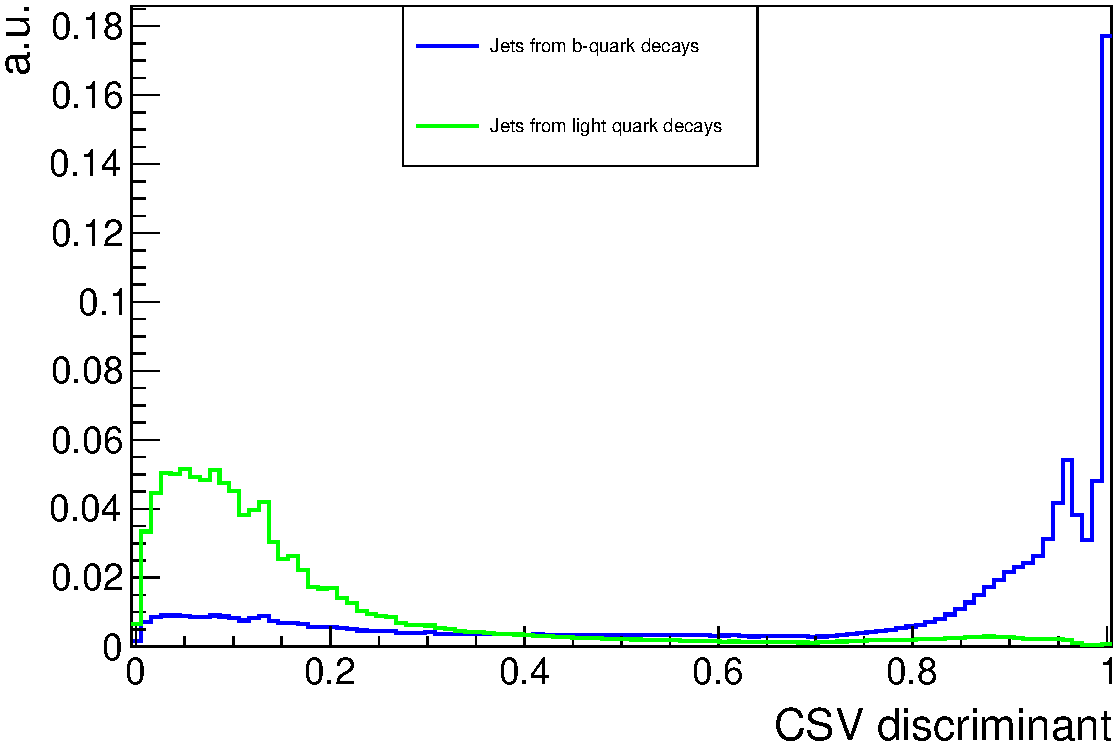
\includegraphics[width = 0.85 \textwidth]{Chapters/Chapter4_EvtSel/Figures/CSVDiscr_LightAndBJets.pdf}
 \caption{CSV discriminant} \label{fig::CSVDiscr}
\end{figure}

\begin{table}[h!t]
 \centering
 \caption{b-tag efficiency for the different working points of the CSV b-tagger.}
 \begin{tabular}{c|c|c|c|c}
  b-tag workin point 	& b-jet efficiency 	& udscg efficiency 	& c-jet efficiency 	& udsg efficiency 	\\
  \hline
  double Loose 		& 83.79 $\%$		& 18.91 $\%$		& 42.44 $\%$ 		& 13.4 $\%$		\\
  double Medium 	& 68.71 $\%$		& 4.57 $\%$		& 18.88 $\%$		& 1.21 $\%$		\\
  double Tight 		& 52.11 $\%$ 		& 1.22 $\%$ 		& 5.74 $\%$ 		& 0.16 $\%$ 		\\
 \end{tabular}
\end{table}


Since in this analysis emphasis lies on the correct reconstruction of the event topology, the choice of the b-tag working point has been based on the efficiency to precisely select the four jets present in the event. Hence, as was to be expected, the requirement of having at least two of these jets to be tagged using the most stringent working point results in the optimal reconstruction efficiency. As an additional bonus, this significantly reduces the event rates such that this additional event selection constraint also has a beneficial effect on the required processing time.
\\
With the b-tag working point fixed, the topology reconstruction proceeds by assigning the two most energetic jets surviving the b-tag requirement to the two jets originating from the b-quark decay. All other jets are then labelled as ``light jets'' and will need to be appointed \textbf{to the two} remaining jets in the event. 
In order to increase the efficiency of identifying the two correct light jets in the event the topology reconstruction has been adapted to consider the three most energetic light jets, if available, and assign the two most plausible ones to the jets produced during the hadronic decay of one of the W-bosons.
This choice again improves the topology reconstruction efficiency since for a significant number of events this third light jet is actually one of the correct jets.
\\
This light jet selection procedure is based on a $\chi^{2}$ method using both the mass of the lepton and the leptonic b and the mass of the hadronic b together with the two light quarks. Hence, this allows to, beside determining the two light jets, simultaneously distinguish the b-jet originating from the hadronic and the leptonic decaying top quark.
The expected values for both masses, denoted as $M_{lb}$ and $M_{qqb}$ respectively, have been determined using the semi-leptonically decaying top quarks with only the main event/the full event selection discussed up to now applied.\footnote{ (\textit{Why do you determine this before the b-tag? The b-tag will significantly influence the obtained mass values ... but will also reduce the available statistics ...} \textbf{Actually have also determined these values after the b-tags and the difference is almost negligible ...})}
The selection procedure then selects the event configuration for which these two mass values correspond the most with the expected values, taking into account their uncertainties.
\begin{equation}
 \chi^{2}_{M_{lb}, M_{qqb}} = \frac{(\hat{M_{lb}} - M_{lb})^{2}}{\sigma^{2}(\hat{M_{lb}})} + \frac{(\hat{M_{qqb}} - M_{qqb})^{2}}{\sigma^{2}(\hat{M_{qqb}})}
\end{equation}

An important motivation to use the $M_{lb}$ value in stead of the more obvious leptonic topquark mass is related to the difficult reconstruction of the neutrino.
Since only information on the $z$-component of this particle is available in particle detectors requires the determination of the $x$- and $y$-component the use of complex calculations based on the reconstructed masses. As a result it would not make much sense to reconstruct this particle, using the mass information, for then only using the leptonical top-quark mass. Especially since the $M_{lb}$ value can easily be reconstructed and fitted, although attention should be awarded to restrict the range where the fit is applied since this distribution is not expected to demonstrate the perfect Gaussian behaviour expected for the top quark mass.

\begin{table}[h!t]
 \centering
 \begin{tabular}{c|c|c|c}
		& $\hat{M_{lb}}$ ($\GeV$) 	& $\hat{M_{qqb}}$ ($\GeV$) 	& $\hat{M_{W}}$ ($\GeV$) 	\\
  \hline
  no b-tag 	& 106.9388 $\pm$ 32.0410 	& 174.5792 $\pm$ 17.5196 	& 83.7810 $\pm$ 10.2311 	\\
  b-tag 	& 107.7945 $\pm$ 32.4255 	& 175.0311 $\pm$ 17.0589 	& 83.6161 $\pm$ 10.2171 	
 \end{tabular}
 \caption{Obtained masses from Gaussian fit on distribution obtained before and after the application of the b-tagging requirement.}
\end{table}

Line
\\
\\
\textit{It is here that the choice of the two light jets takes place, in case of more than three light jets being present in the event!}\\
\textit{Will need to recalculate the numbers for the different b-tag options since the definition of light jets has changed ...} \\
\textit{And will also need to get these numbers for muon channel events alone ... Currently everything is done for muon and electron channel combined!}
\\
\\
\newpage
\paragraph{\underline{Comparing the 4 and 5 jet case for all the b-tags:}}
\subsubsection{4-jet case}
\begin{table}[!h] 
 \begin{tabular}{c|c|c|c|c|c} 
  \textbf{Option} & all 4 correct & $\geq$ 1 wrong       & correct ($\%$)       & $\frac{s}{b}$ & non-matched \\ \hline 
  2 L b-tags              & 426636 & 612386 & 41.0613 & 0.696678 & 1568843\\ 
  %2 L b-tags, light L-veto & 345646 & 487775 & 41.4732 & 0.708618 & 1268935\\ 
  2 M b-tags              & 325578 & 327020 & 49.8895 & 0.995591 & 826872\\ 
  %2 M b-tags, light M-veto & 310201 & 306237 & 50.3215 & 1.01294 & 783840\\ 
  %2 M b-tags, light L-veto & 237042 & 262674 & 47.4353 & 0.902419 & 625001\\ 
  2 T b-tags              & 198204 & 162941 & 54.8821 & 1.21642 & 422919\\ 
  %2 T b-tags, light T-veto & 195569 & 159603 & 55.0632 & 1.22535 & 415450\\ 
  %2 T b-tags, light M-veto & 181012 & 155451 & 53.7985 & 1.16443 & 394155\\ 
  %2 T b-tags, light L-veto & 138583 & 137450 & 50.2052 & 1.00824 & 317064\\ 
 \end{tabular} 
 \caption{Overview of correct and wrong reconstructed events for the different b-tags (no $\chi^{2}$ $m_{lb}$ - $m_{qqb}$ applied)}
\end{table} 
 
\begin{table}[!h] 
 \begin{tabular}{c|c|c|c|c|c} 
  \textbf{Option} & 2 b's correct & $\geq$ 1 b wrong     & b's correct ($\%$)   & $\frac{s}{b}$ & non-matched \\ \hline 
  2 L b-tags              & 589953 & 449069 & 56.7796 & 1.31372 & 1568843\\ 
  %2 L b-tags, light L-veto & 500672 & 332749 & 60.0743 & 1.50465 & 1268935\\ 
  2 M b-tags              & 460691 & 191907 & 70.5934 & 2.4006 & 826872\\ 
  %2 M b-tags, light M-veto & 445064 & 171374 & 72.1993 & 2.59703 & 783840\\ 
  %2 M b-tags, light L-veto & 360899 & 138817 & 72.2208 & 2.59982 & 625001\\ 
  2 T b-tags              & 280306 & 80839 & 77.6159 & 3.46746 & 422919\\ 
  %2 T b-tags, light T-veto & 277571 & 77601 & 78.1511 & 3.5769 & 415450\\ 
  %2 T b-tags, light M-veto & 263210 & 73253 & 78.2285 & 3.59316 & 394155\\ 
  %2 T b-tags, light L-veto & 213584 & 62449 & 77.3763 & 3.42013 & 317064\\ 
 \end{tabular} 
 \caption{Overview of correct and wrong reconstructed b-jets for the different b-tags (no $\chi^{2}$ $m_{lb}$ - $m_{qqb}$ applied)}
\end{table} 
 
\begin{table}[!h] 
 \begin{tabular}{c|c|c|c|c|c} 
  \textbf{Option} & 2 light good  & $\geq$ 1 light wrong & light correct ($\%$) & $\frac{s}{b}$ & non-matched \\ \hline 
  2 L b-tags              & 504181 & 534841 & 48.5246 & 0.942675 & 1568843\\ 
  %2 L b-tags, light L-veto & 415812 & 417609 & 49.8922 & 0.995697 & 1268935\\ 
  2 M b-tags              & 374193 & 278405 & 57.339 & 1.34406 & 826872\\ 
  %2 M b-tags, light M-veto & 358096 & 258342 & 58.0912 & 1.38613 & 783840\\ 
  %2 M b-tags, light L-veto & 274331 & 225385 & 54.8974 & 1.21717 & 625001\\ 
  2 T b-tags              & 227716 & 133429 & 63.0539 & 1.70665 & 422919\\ 
  %2 T b-tags, light T-veto & 225072 & 130100 & 63.3699 & 1.72999 & 415450\\ 
  %2 T b-tags, light M-veto & 209171 & 127292 & 62.1676 & 1.64324 & 394155\\ 
  %2 T b-tags, light L-veto & 160090 & 115943 & 57.9967 & 1.38076 & 317064\\ 
 \end{tabular} 
 \caption{Overview of correct and wrong reconstructed light jets for the different b-tags (no $\chi^{2}$ $m_{lb}$ - $m_{qqb}$ applied)}
\end{table} 

\newpage
\subsubsection{5-jet case}
\begin{table}[!h] 
 \begin{tabular}{c|c|c|c|c|c} 
  \textbf{Option} & all 4 correct & $\geq$ 1 wrong       & correct ($\%$)       & $\frac{s}{b}$ & non-matched \\ \hline 
  2 L b-tags              & 512367 & 526655 & 49.3124 & 0.97287 & 1568843\\ 
  %2 L b-tags, light L-veto & 410486 & 422935 & 49.2531 & 0.970565 & 1268935\\ 
  2 M b-tags              & 396904 & 255694 & 60.8191 & 1.55226 & 826872\\ 
  %2 M b-tags, light M-veto & 377217 & 239221 & 61.193 & 1.57686 & 783840\\ 
  %2 M b-tags, light L-veto & 282672 & 217044 & 56.5665 & 1.30237 & 625001\\ 
  2 T b-tags              & 241394 & 119751 & 66.8413 & 2.0158 & 422919\\ 
  %2 T b-tags, light T-veto & 238024 & 117148 & 67.0165 & 2.03182 & 415450\\ 
  %2 T b-tags, light M-veto & 219617 & 116846 & 65.2723 & 1.87954 & 394155\\ 
  %2 T b-tags, light L-veto & 164817 & 111216 & 59.7092 & 1.48195 & 317064\\ 
 \end{tabular} 
 \caption{Overview of correct and wrong reconstructed events for the different b-tags (no $\chi^{2}$ $m_{lb}$ - $m_{qqb}$ applied, 5 jets considered)}
\end{table} 
 
\begin{table}[!h] 
 \begin{tabular}{c|c|c|c|c|c} 
  \textbf{Option} & 2 b's correct & $\geq$ 1 b wrong     & b's correct ($\%$)   & $\frac{s}{b}$ & non-matched \\ \hline 
  2 L b-tags              & 589953 & 449069 & 56.7796 & 1.31372 & 1568843\\ 
  %2 L b-tags, light L-veto & 500672 & 332749 & 60.0743 & 1.50465 & 1268935\\ 
  2 M b-tags              & 460691 & 191907 & 70.5934 & 2.4006 & 826872\\ 
  %2 M b-tags, light M-veto & 445064 & 171374 & 72.1993 & 2.59703 & 783840\\ 
  %2 M b-tags, light L-veto & 360899 & 138817 & 72.2208 & 2.59982 & 625001\\ 
  2 T b-tags              & 280306 & 80839 & 77.6159 & 3.46746 & 422919\\ 
  %2 T b-tags, light T-veto & 277571 & 77601 & 78.1511 & 3.5769 & 415450\\ 
  %2 T b-tags, light M-veto & 263210 & 73253 & 78.2285 & 3.59316 & 394155\\ 
  %2 T b-tags, light L-veto & 213584 & 62449 & 77.3763 & 3.42013 & 317064\\ 
 \end{tabular} 
 \caption{Overview of correct and wrong reconstructed b-jets for the different b-tags (no $\chi^{2}$ $m_{lb}$ - $m_{qqb}$ applied, 5 jets considered)}
\end{table} 
 
\begin{table}[!h] 
 \begin{tabular}{c|c|c|c|c|c} 
  \textbf{Option} & 2 light good  & $\geq$ 1 light wrong & light correct ($\%$) & $\frac{s}{b}$ & non-matched \\ \hline 
  2 L b-tags              & 603601 & 435421 & 58.0932 & 1.38625 & 1568843\\ 
  %2 L b-tags, light L-veto & 493376 & 340045 & 59.1989 & 1.45091 & 1268935\\ 
  2 M b-tags              & 452953 & 199645 & 69.4077 & 2.26879 & 826872\\ 
  %2 M b-tags, light M-veto & 432443 & 183995 & 70.1519 & 2.3503 & 783840\\ 
  %2 M b-tags, light L-veto & 324766 & 174950 & 64.9901 & 1.85634 & 625001\\ 
  2 T b-tags              & 275125 & 86020 & 76.1813 & 3.19838 & 422919\\ 
  %2 T b-tags, light T-veto & 271763 & 83409 & 76.5159 & 3.2582 & 415450\\ 
  %2 T b-tags, light M-veto & 251381 & 85082 & 74.7128 & 2.95457 & 394155\\ 
  %2 T b-tags, light L-veto & 188773 & 87260 & 68.3878 & 2.16334 & 317064\\ 
 \end{tabular} 
 \caption{Overview of correct and wrong reconstructed light jets for the different b-tags (no $\chi^{2}$ $m_{lb}$ - $m_{qqb}$ applied, 5 jets considered)}
\end{table} 
 

\newpage
\subsection{Number of light jets}

\subsection{Signal optimisation}\label{subsec::MassCuts}

\subsection{Data-MC agreement}\label{subsec::DataMC}